\documentclass[12pt]{article}
\usepackage{homework}
\pagestyle{fancy}

% assignment information
\def\course{Thermodynamics}
\def\assignmentno{Problem Set 2}
\def\assignmentname{First and Second Law \& Associated Reasoning}
\def\name{Xin, Wenkang}
\def\time{\today}

\begin{document}

\begin{titlepage}
    \begin{center}
        \large
        \textbf{\course}

        \vfill

        \Huge
        \textbf{\assignmentno}

        \vspace{1.5cm}

        \large{\assignmentname}

        \vfill

        \large
        \name

        \time
    \end{center}
\end{titlepage}


%==========
\pagebreak
\section*{Energy}
%==========


\problem{A.1}{}
For a straight-line path, pressure $p$ and volume $V$ are related by:

\begin{equation}
    p(V) = \frac{p_{2} - p_{1}}{V_{2} - V_{1}} V + \frac{p_{1} V_{2} - p_{2} V_{1}}{V_{2} - V_{1}}
\end{equation}

The work done on the gas is:

\begin{equation}
    W = -\int_{V_{1}}^{V_{2}} p \, \mathrm{d}V = -\int_{V_{1}}^{V_{2}} \left( \frac{p_{2} - p_{1}}{V_{2} - V_{1}} V + \frac{p_{1} V_{2} - p_{2} V_{1}}{V_{2} - V_{1}} \right) \, \mathrm{d}V = \frac{1}{2} (p_{1} + p_{2}) (V_{1} - V_{2})
\end{equation}

We know that $\gamma = C_{p} / C_{V}$ and $C_{p} - C_{V} = nR$ for an ideal gas. Therefore, we have $C_{V} = nR / (\gamma - 1)$. The change in internal energy is:

\begin{equation}
    \Delta U = C_{V} \Delta T = \frac{nR}{\gamma - 1} \Delta T
\end{equation}

By the first law of thermodynamics, we have:

\begin{equation}
    Q = \Delta U - W = \frac{nR}{\gamma - 1} \Delta T + \frac{1}{2} (p_{1} + p_{2}) (V_{2} - V_{1})
\end{equation}

Substituting the numbers, we have $W = \qty{-120}{J}$, $\Delta U = \qty{831}{J}$ and $Q = \qty{951}{J}$.
\qed


\problem{A.2}{}
In an adiabatic process, we have $p \mathrm{d}V = -\mathrm{d}U = -C_{V} \mathrm{d}T$. On the other hand, the ideal gas law gives $p = nRT/V$. Therefore, we have:

\begin{equation}
\begin{split}
    \frac{nRT}{V} \mathrm{d}V &= -C_{V} \mathrm{d}T \\
    \frac{nR}{C_{V}} \frac{\mathrm{d}V}{V} &= -\frac{\mathrm{d}T}{T} \\
    (\gamma - 1) \ln V &= -\ln T + C \\
    \ln{\left( TV^{\gamma - 1} \right)} &= C \\
    TV^{\gamma - 1} &= C
\end{split}
\end{equation}

Using the ideal gas law, we have $pV = nRT$. Therefore, we have:

\begin{equation}
    pV^{\gamma} = C
\end{equation}

and:

\begin{equation}
    T^{\gamma} p^{1 - \gamma} = C
\end{equation}
\qed


\problem{A.3}{}
In an adiabatic expansion, we have the work done on the gas:

\begin{equation}
    W = -\int_{V_{1}}^{V_{2}} p \, \mathrm{d}V = -\int_{V_{1}}^{V_{2}} C V^{-\gamma} \, \mathrm{d}V = \frac{C}{1 - \gamma} \left( V_{2}^{1 - \gamma} - V_{1}^{1 - \gamma} \right)
\end{equation}

But the constant $C$ is given by $C = p_{1} V_{1}^{\gamma}$. Therefore, we have:

\begin{equation}
    W = \frac{p_{1}V_{1}}{\gamma - 1} \left[ \left( \frac{V_{1}}{V_{2}} \right)^{\gamma - 1} - 1 \right]
\end{equation}
\qed


\problem{A.4}{}
In the adiabatic expansion, the work done on the gas is:

\begin{equation}
    W = \frac{p_{1}V_{1}}{\gamma - 1} \left[ \left( \frac{V_{1}}{V_{2}} \right)^{\gamma - 1} - 1 \right] = \frac{nRT_{1}}{\gamma - 1} \left[ \left( \frac{V_{1}}{V_{2}} \right)^{\gamma - 1} - 1 \right] = \qty{-111}{J}
\end{equation}

The heat absorbed during the isochoric process can be calculated using the first law:

\begin{equation}
    Q = \Delta U - W = C_{V} \Delta T - W = \qty{942}{J}
\end{equation}
\qed


\problem{A.5}{}
The Young's modulus can be calculated as:

\begin{equation}
\begin{split}
    E &= \frac{L_{0}}{A} \frac{\partial f}{\partial L} \\
    &= \frac{KTL_{0}}{A} \frac{\partial}{\partial L} \left( \frac{L}{L_{0}} - \frac{L_{0}^{2}}{L^{2}} \right) \\
    &= \frac{KTL_{0}}{A} \left( \frac{1}{L_{0}} + \frac{2L_{0}^{2}}{L^{3}} \right) \\
    &= \frac{KT}{A} \left( 1 + 2 \frac{L_{0}^{3}}{L^{3}} \right)
\end{split}
\end{equation}

The work required to stretch the substance isothermally is:

\begin{equation}
    W = \int_{L_{0}}^{2L_{0}} f \, \mathrm{d}L = KT \int_{L_{0}}^{2L_{0}} \left( \frac{L}{L_{0}} - \frac{L_{0}^{2}}{L^{2}} \right) \, \mathrm{d}L = KTL_{0}
\end{equation}
\qed


\problem{A.6}{}

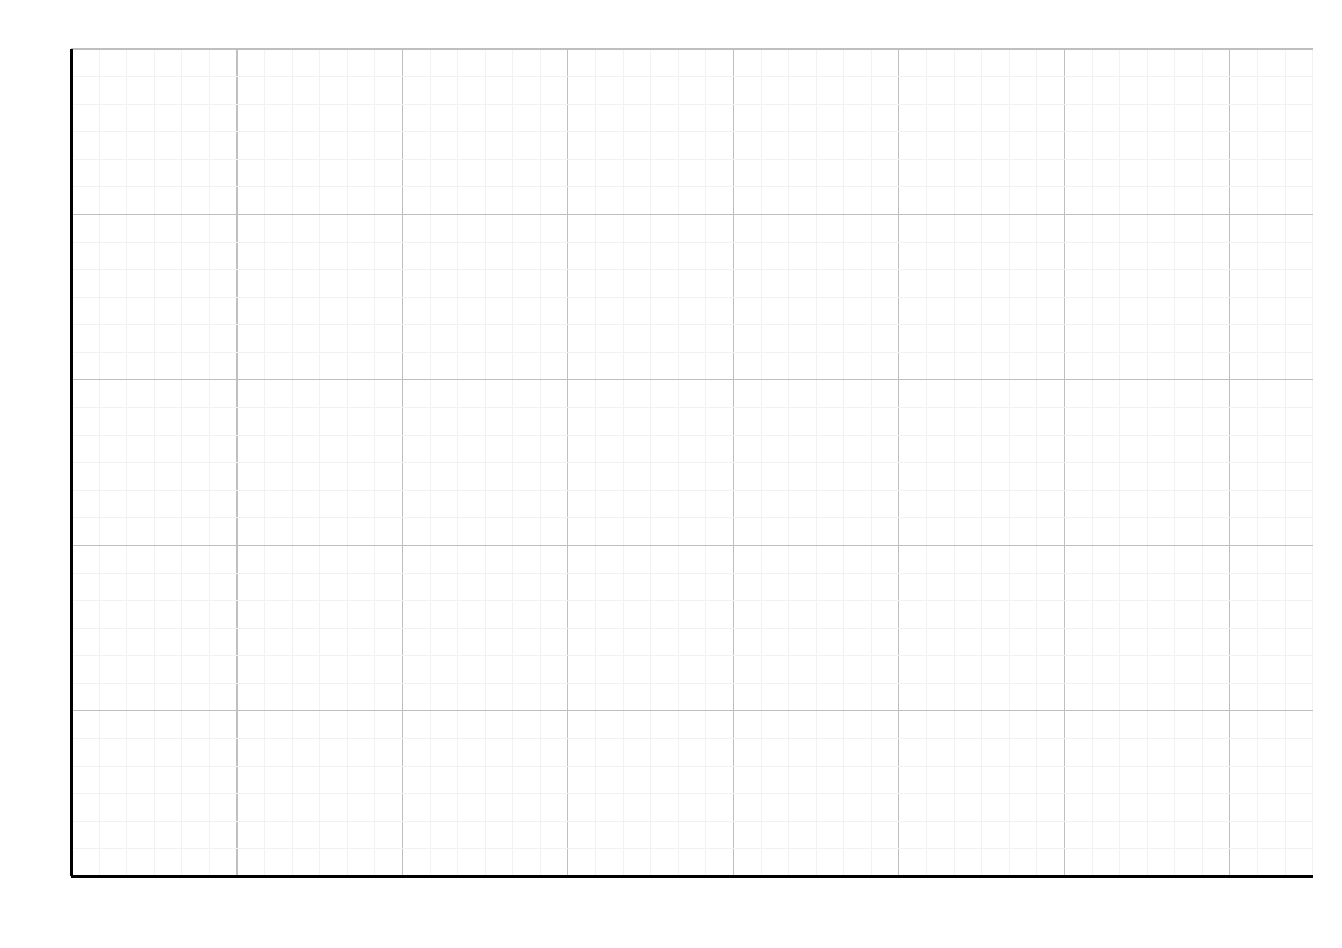
\begin{tikzpicture}[scale = 2.3]
\begin{axis}[
    title = ,
    xmin=0, xmax=15,
    ymin=0, ymax=10,
    grid=both,
    grid style={line width=.1pt, draw=gray!10},
    major grid style={line width=.2pt,draw=gray!50},
    axis lines*=middle,
    minor tick num=5,
    xtick style={draw=none},ytick style={draw=none},
    xticklabels={, ,},yticklabels={, ,},
    axis equal image
    ]
\end{axis}
\end{tikzpicture}
\qed


\problem{A.7}{}
When the pressure equalise, the gas inside the chamber, whose volume we denote as $V_{0}$, will have a temperature $T_{f}$, pressure $p_{0}$ and some number of moles $n_{0}$. These variables are related by the ideal gas law $p_{0}V_{0} = n_{0}RT_{f}$. 

In the process of the gas entering the chamber, the ideal gas law reads $pV = nRT$, so that $p/p_{0} = nT/n_{0}T_{f}$. The infinitesimal work done on the gas is:

\begin{equation}
    \mathrm{d}W = (p_{0} - p) \, \mathrm{d}\tau = p_{0} \left( 1 - \frac{nT}{n_{0}T_{f}} \right) \, \mathrm{d}\tau = \frac{p_{0}}{\rho} \left( 1 - \frac{nT}{n_{0}T_{f}} \right) \, \mathrm{d}n
\end{equation}

where $\mathrm{d}n$ is the infinitesimal number of moles of gas entering the chamber and $\rho = p_{0}/RT_{0}$ is the density of the gas outside the chamber.

To solve this, it remains to find an expression $T(n)$ for the temperature of the gas inside. First law gives:

\begin{equation}
\begin{split}
    C_{V} T &= C_{V} T_{0} + W \\
    T &= T_{0} + \frac{\gamma - 1}{nR} W
\end{split}
\end{equation}

Substituting, we have the equation:

\begin{equation}
    \frac{\mathrm{d}W}{\mathrm{d}n} = \frac{p_{0}}{\rho} \left[ 1 - \frac{nT_{0} + (\gamma - 1)W/R}{n_{0}T_{f}} \right] = \kappa - An - BW
\end{equation}

where $\kappa = p_{0}/\rho$, $A = p_{0}T_{0}/\rho n_{0}T_{f}$ and $B = (\gamma - 1)p_{0}/\rho n_{0}RT_{f}$. This is a first order linear differential equation. Solving the equation and requiring that $W(n = 0) = 0$, we have:

\begin{equation}
    W(n) = (A + B\kappa) \left( \frac{1}{B^{2}} - e^{Bn} \right) - \frac{A}{B}n
\end{equation}

Substituting this into the equation for $T(n)$, we have:

\begin{equation}
    T_{f} = T_{0} + \frac{\gamma - 1}{n_{0} R} W(n_{0})
\end{equation}

which can be solved to give:

\begin{equation}
    T_{f} = \frac{\gamma - 1}{\ln{\gamma}} T_{0}
\end{equation}
\qed


%==========
\pagebreak
\section*{Second Law and Entropy}
%==========


\problem{B.1}{}
This is possible as the process is not cyclic. 

Kelvin's statement of the second law of thermodynamics states it it impossible to have a cyclic process that converts heat completely into work. However, this process is not cyclic and therefore does not violate the second law of thermodynamics.
\qed


\problem{B.2}{}
First suppose that Clausius' statement is true. If Kelvin's statement is false, then it is possible to have a cyclic machine $E$ that completely converts $Q$ supplied to it to work $W = Q$. Consider a heat pump that takes in $Q_{2}$ from a cold reservoir and some work $W$, releasing $Q_{1} = Q_{2} + W$ to a hot reservoir. We can arrange the engines such that the work $W$ is supplied by $E$ which draws heat $Q = W$ from the cold reservoir. Then this is a process that moves heat from a cold reservoir to a hot reservoir without any other effect. This violates Clausius' statement and therefore Kelvin's statement must be true if Clausius' holds.

Next suppose that Kelvin's statement is true. If Clausius' statement is false, then it is possible to have a process that moves heat from a cold reservoir to a hot reservoir without any other effect. Let this process be realised by a machine $M$ that takes heat $Q$ from a cold reservoir to a hot reservoir. Consider an engine that takes heat $Q_{1}$ from a hot reservoir and releases heat $Q_{2}$ to a cold reservoir, producing work $W = Q_{1} - Q_{2}$ in the process. We can use the machine $M$ to move heat $Q_{2}$ from the cold reservoir back to the hot reservoir. This is a cyclic process that converts heat completely into work, violating Kelvin's statement. Therefore, Clausius' statement must be true if Kelvin's holds.

The above arguments show that Kelvin's statement and Clausius' statement are equivalent.
\qed


\problem{B.3}{}
The rate of heat loss must be compensated by the rate of heat supply by the heat pump. By the first law of thermodynamics, we have:

\begin{equation}
    P_{1} = \alpha(T - T_{0}) = W + P_{2}
\end{equation}

where $P_{1}$ is the rate of heat supply and $P_{2}$ is the rate of heat drawing from the cold reservoir (river).

For an ideal heat pump, we have $P_{2}/P_{1} = T_{0}/T$. Therefore, we solve the following second order equation for $T$:

\begin{equation}
\begin{split}
    \alpha(T - T_{0}) = W + \frac{T_{0}}{T} \alpha(T - T_{0})
\end{split}
\end{equation}

which has the solution:

\begin{equation}
    T = T_{0} + \frac{W}{2\alpha} \left( 1 + \sqrt{1 + \frac{4\alpha T_{0}}{W}} \right)
\end{equation}

where the negative solution is discarded as it is unphysical.
\qed


\problem{B.4}{}
For the given cycle, the heat intake happens at the second step, an isochoric expansion:

\begin{equation}
    Q_{\text{in}} = \Delta U_{2} = \frac{nR}{\gamma - 1} \Delta T = \frac{1}{\gamma - 1} (p_{2}V_{2} - p_{1}V_{2})
\end{equation}

The heat exhaust happens at the first step, an isobaric compression:

\begin{equation}
    Q_{\text{out}} = W - \Delta U_{1} = p_{1}(V_{1} - V_{2}) + \frac{1}{\gamma - 1} (p_{1}V_{1} - p_{1}V_{2})
\end{equation}

Work is done by the gas at the third step, an adiabatic expansion:

\begin{equation}
    W = \frac{p_{2}V_{2}}{\gamma - 1} \left[ 1 - \left( \frac{V_{2}}{V_{1}} \right)^{\gamma - 1} \right]
\end{equation}

The thermal efficiency is:

\begin{equation}
    \eta = \frac{W}{Q_{\text{in}}} = \frac{p_{2}V_{2}}{\gamma - 1} \left[ 1 - \left( \frac{V_{2}}{V_{1}} \right)^{\gamma - 1} \right] \frac{\gamma - 1}{p_{2}V_{2} - p_{1}V_{2}} = \frac{p_{2}}{p_{2} - p_{1}} \left[ 1 - \left( \frac{V_{2}}{V_{1}} \right)^{\gamma - 1} \right]
\end{equation}

But the fact that $p_{1}V_{1}^{\gamma} = p_{2}V_{2}^{\gamma}$ gives:
\qed


\problem{B.5}{}
The entropy change of the tea cooling down is:

\begin{equation}
    \Delta S = \int_{T_{0}}^{T_{f}} \frac{mc}{T} \, \mathrm{d}T = -mc \ln{\frac{T_{0}}{T_{f}}} = \qty{-185.6}{JK^{-1}}
\end{equation}

The negative sign indicates that the entropy of the tea decreases as it cools down.
\qed


\problem{B.6}{}
Consider a negative $\delta Q$. Since $T$ expressed in Kelvin is always positive, we may have a positive $\Delta S$ with opposite sign to $\delta Q$.
\qed


\problem{B.7}{}

\subproblem{a}
The entropy change of the block is:

\begin{equation}
    \Delta S_{b} = \int_{T_{0}}^{T_{f}} \frac{C}{T} \, \mathrm{d}T = C \ln{\frac{T_{f}}{T_{0}}} = \qty{-41.4}{JK^{-1}}
\end{equation}

The entropy change of the lake is:

\begin{equation}
    \Delta S_{l} = \int \frac{1}{T_{0}} \, \mathrm{d}Q = C \frac{T_{f} - T_{0}}{T_{0}} = \qty{47.7}{JK^{-1}}
\end{equation}

so that the total entropy change is:

\begin{equation}
    \Delta S_{\text{uni}} = \Delta S_{b} + \Delta S_{l} = \qty{6.3}{JK^{-1}}
\end{equation}

\subproblem{b}
In addition to the above entropies, the gravitational potential energy of the block is converted to kinetic energy and then to heat of the lake. The entropy change of the block is the same as before. The entropy change of the lake changes to:

\begin{equation}
    \Delta S_{l} =C \frac{T_{f} - T_{0}}{T_{0}} + \frac{mgh}{T_{0}} = \qty{47.7}{Jk^{-1}} + \qty{0.1}{Jk^{-1}} = \qty{49.1}{JK^{-1}}
\end{equation}

so that the total entropy change is:

\begin{equation}
    \Delta S_{\text{uni}} = \Delta S_{b} + \Delta S_{l} = \qty{7.7}{JK^{-1}}
\end{equation}

\subproblem{c}
The final temperature of the block satisfies:

\begin{equation}
    C(T_{100} - T_{f}) = C(T_{f} - T_{10})
\end{equation}

so that $T_{f} = \qty{55}{\degree C}$.

The total entropy change is:

\begin{equation}
    \Delta S_{\text{uni}} = \Delta S_{1} + \Delta S_{2} = C \ln{\frac{T_{f}}{T_{10}}} + C \ln{\frac{T_{f}}{T_{100}}} = \qty{2.8}{JK^{-1}}
\end{equation}

\subproblem{d}
In any real circuit there is a resistance $R$ and the power dissipated is $P = I^{2}R$, where the current is given by the transient solution:

\begin{equation}
    I(t) = \frac{V}{R} e^{-t/RC}
\end{equation}


The charging is fast such that there is effectively no temperature change. The only place where heat is concerned is the resistor. The entropy change of the resistor is:

\begin{equation}
    \Delta S_{R} = \int \frac{1}{T} \, \mathrm{d}Q = \int \frac{1}{T} I^{2} R \, \mathrm{d}t = \frac{V^{2}}{RT} \int_{0}^{\infty} e^{-2t/RC} \, \mathrm{d}t = \frac{CV^{2}}{2T} = \qty{1.83e-5}{JK^{-1}}
\end{equation}

which is just the total entropy change.

\subproblem{e}
The entropy change is the same as before, as the same amount of electric field energy $CV^{2}/2$ is dissipated as heat in the resistor.

\subproblem{f}
For a reversible and isothermal expansion:

\begin{equation}
    \Delta S = \int \frac{\mathrm{d}Q}{T} = \int \frac{p \mathrm{d}V}{T} = \int \frac{nRT}{V} \frac{\mathrm{d}V}{T} = nR \ln{\frac{V_{f}}{V_{i}}} = \qty{5.76}{JK^{-1}}
\end{equation}

\subproblem{g}
For a reversible and adiabatic expansion, there is no heat exchange and therefore no entropy change.
\qed

\end{document}